\documentclass[11pt,singlespacing,liststotoc,headsepline,a4paper]{article}

%Librerias, simbolos, idioma, paginación
%\usepackage[spanish,es-tabla,es-lcroman,es-noindentfirst,es-nosectiondot,es-nodecimaldot]{babel}
\usepackage[utf8]{inputenc} % Required for inputting international characters
\usepackage[T1]{fontenc} % Output font encoding for international characters
%\usepackage{fancyhdr}
%\usepackage{mhchem} %Para formulas quimicas (sobretodo el problema de subindices)


%Librerias imagenes
\usepackage{graphicx}
\graphicspath{ {Figures/} }
\usepackage[justification=centering]{caption}
\usepackage{float}
\usepackage{rotating} %rotación de tablas

%Libreria refencias
\usepackage[backend=bibtex,natbib=true]{biblatex} % Use the bibtex backend with the authoryear citation style (which resembles APA)
\addbibresource{References.bib} % The filename of the bibliography
\usepackage[autostyle=true]{csquotes} % Required to generate language-dependent quotes in the bibliography

%Librerias matematicas
\usepackage{mathtools} %%%Quitar este???
\usepackage{amssymb, amsmath, amsbsy} 

%Otras
%\usepackage{hyperref}% Hipervinculos
\usepackage{multirow}% Tablas
%\usepackage[bookmarks = true, colorlinks=true, linkcolor = black, citecolor = black, menucolor = black, urlcolor = black]{hyperref} 
\usepackage{mathpazo} % Use the Palatino font by default
\usepackage{afterpage}

%opening
\title{\textsc{\Huge Entrega 1: Análisis numérico de un cambio de órbita de un satélite}}

\author{
	Alejando Fernández Herrero\\
	\and
	Ángel Luis Porras Hermoso\\
	\and
	Raúl Moreno Ginés
}

\date{\today}


\begin{document}

\medskip
\vfill
{\let\newpage\relax\maketitle}
\vfill
\medskip
\thispagestyle{empty}
\clearpage

\newpage

\begin{abstract}
	
En este informe se recogen aquellos trabajos e hitos que se han planteado durante el primer semestre de 1º de MUSE de 2018. Se plantean los problemas y ejercicios propuestos así como la metodología seguida para el diseño de software de los programas implicados. Adicionalmente se  plantea estudiar el impacto que sufre en la órbita de diseño un satélite al que le falle el control de apagado del motor cohete eléctrico, para analizar el riesgo e impacto que este tipo de fallo tendría en una hipotética misión.\\

\end{abstract}

\thispagestyle{empty}
\clearpage

\newpage
\tableofcontents % Prints the main table of contents
\newpage
\listoffigures
\thispagestyle{empty}
\clearpage

\renewcommand{\thepage}{\arabic{page}}
\setcounter{page}{1}

	\newpage

\section{Introducción}
El cambio de órbita de un satélite es una maniobra necesaria en la puesta en órbita de un satélite. Este cambio de órbita permite al sistema cambiar desde una órbita de aparcamiento alcanzable por el lanzador a la órbita final pretendida en el proyecto.

Para realizar correctamente esta maniobra es necesario ejecutar previamente un análisis mediante cálculo numérico. Para este análisis comúnmente se usan distintos lenguajes de programación para reducir el tiempo de cálculo.

A lo largo de este informe se presentarán metodologías de programación y métodos de estimación distintos para optimizar el cálculo numérico. Además, se presentarán una serie de modelos de distintos problemas similares al estudiado y los códigos utilizados para dichos modelos.

	\newpage
	
\section{Modelos numéricos}
Los modelos simulados a lo largo del informe se implementarán usando diferentes esquemas numéricos o propagadores. El principal esquema numérico utilizado es el Runge-Kutta. Este propagador tiene diferentes niveles, que alcanzan precisiones cada vez mayores. Para los análisis preliminares, sin demasiado detalle, se ha empleado el Runge-Kutta de nivel 2, mientras que para análisis más precisos se ha utilizado el Runge-Kutta de nivel 4.

A parte del Runge-Kutta se ha implantado también un esquema numérico de tipo Euler explícito. Este modelo numérico, como se irá viendo a lo largo del informe, presenta problemas de convergencia para determinadas funciones, lo que hará que para obtener resultados lo más precisos posible se recurra a los esquemas del tipo Runge-Kutta.


	\newpage

\section{Metodologías y herramientas de programación}

Todo proyecto software que se quiere llevar a acabo debería seguir los pasos que se propone la Figura \ref{Esquema}:

\begin{figure}[htbp]
	\centering
	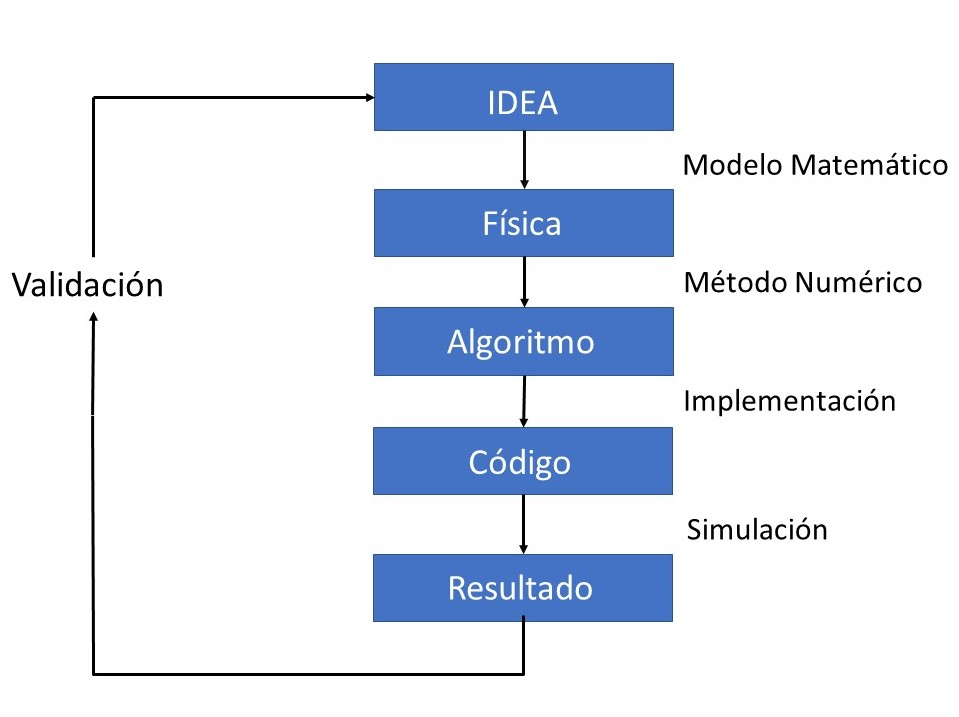
\includegraphics[width=0.6\textwidth]{Esquema.JPG}
	\caption{Esquema de los pasos a seguir en el diseño software}
	\label{Esquema}
\end{figure}

Este esquema nos explica que partiendo de una idea, lo primero que se debe hacer es plantear la física de nuestro problema a través de un modelo matemático. Una vez se ha definido el modelo matemático a usar se pasa al siguiente paso que es decidir el esquema numérico a emplear, como ya se ha comentado antes es esquema numérico será elegido en función del problema que se quiere resolver y la precisión que se quiere obtener. Este paso nos definirá el algoritmo de resolución de nuestro problema. Con los dos elementos anteriormente dichos  se debe implementar el problema en un código. Para este trabajo se ha elegido FORTRAN, Además se ha para mayor claridad del software se ha divido los archivos del programa; por ejemplo se han separado en archivos distintos módulos , unos módulos contienen las subrutinas encargadas de los esquemas numéricos, mientras que otros módulos contienen las funciones de la física de cada problema, finalmente existen otros archivos que relacionan estos dos módulos para resolver el programa. De esta manera se consigue separar la física del método numérico facilitando la compresión del código. Una vez obtenido el código se llevan acabo distintas simulaciones, obteniendo así resultados que deberán ser validados y comparados con la idea original. Este proceso es iterativo y se espera que se repita este proceso hasta obtener unos resultados satisfactorios.

Además de seguir el esquema anteriormente descrito; a lo largo del curso en el que ha tenido cabida este proyecto se han llevado a cabo distintas metodologías de programación que facilitan la labor del equipo de ingenieros a lo largo de la simulación numérica de los distintos modelos.

En el caso de este proyecto, se ha utilizado principalmente la metodología de \textit{Extreme Programming}, que permite agilizar la labor de programación. Esta metodología consiste en dividir los equipos de programación en \textit{Drivers}, los encargados de redactar el código, y \textit{Reviewers}, encargados de contrastar lo que escriben los \textit{Drivers} y detectar posibles errores en el código. Este sistema permite detectar con mayor facilidad erratas a lo largo de una secuencia de programación y realizar simultáneamente las labores de escritura y revisión. Además, al estar los \textit{Reviewers} constantemente revisando el código, estos ingenieros, o programadores, van asimilando el código.

Dentro de las herramientas de programación destacan la técnica \textit{top-down} y la técnica de continuación.

La técnica de continuación permite llegar a la solución de un problema complejo partiendo de un problema más sencillo a través de herramientas matemáticas. Esta herramienta permite simular, en primeras aproximaciones, problemas complejos con físicas difíciles de implementar descomponiéndolos en problemas más sencillos de implementar.

La técnica \textit{top-down} permite la resolución de un problema compuesto de distintos componentes mediante la descomposición y análisis de esos subsistemas. Esta herramienta es útil para poder reutilizar partes del código para distintos problema, ya que al programar cada parte del sistema en una subrutina diferente, permite llamar a dichas partes del código desde distintos códigos principales para la simulación de diferente modelos.

Como ya se ha comentado anteriormente, se ha decidido usar el lenguaje de programación FORTRAN para este análisis. La utilización de este lenguaje implica el uso de las librerías \textit{dislin} para la representación de gráficas. Las librerías utilizadas no son las propias de \textit{dislin}, sino que se ha utilizado una modificación realizada por nuestro compañero Imanol Sardón Delgado, que nos las ha cedido para su uso. Esta librería permite incluir fácilmente distintos colores en las gráficas, así como títulos de gráfica y de eje y leyendas.

	\newpage
	
\section{Ecuaciones de Bessel}
Como primer paso en este curso se realizó el análisis de las funciones de Bessel, una de las funciones más estudiadas en la parte analítica de la asignatura dentro de la que esta englobada este estudio.

Este problema, aunque sencillo, permite familiarizarse con el entorno de programación utilizado, así como el uso de la herramienta \textit{dislin} para la representación de gráficas. Además, se utilizará este ejemplo para validar los esquemas numéricos. La función de Bessel es el resultado de la siguiente ecuación diferencial ordinaria de orden dos:

\begin{equation}
z ^ { 2 } \frac { \mathrm { d } ^ { 2 } w } { \mathrm { d } z ^ { 2 } } ( z ) + z \frac { \mathrm { d } w } { \mathrm { d } z } ( z ) +  z ^ { 2 }  w ( z ) = 0
\end{equation}



Los resultados obtenidos de este sencillo análisis se presentan en las gráficas a continuación:

\begin{figure}[H]
	\centering
	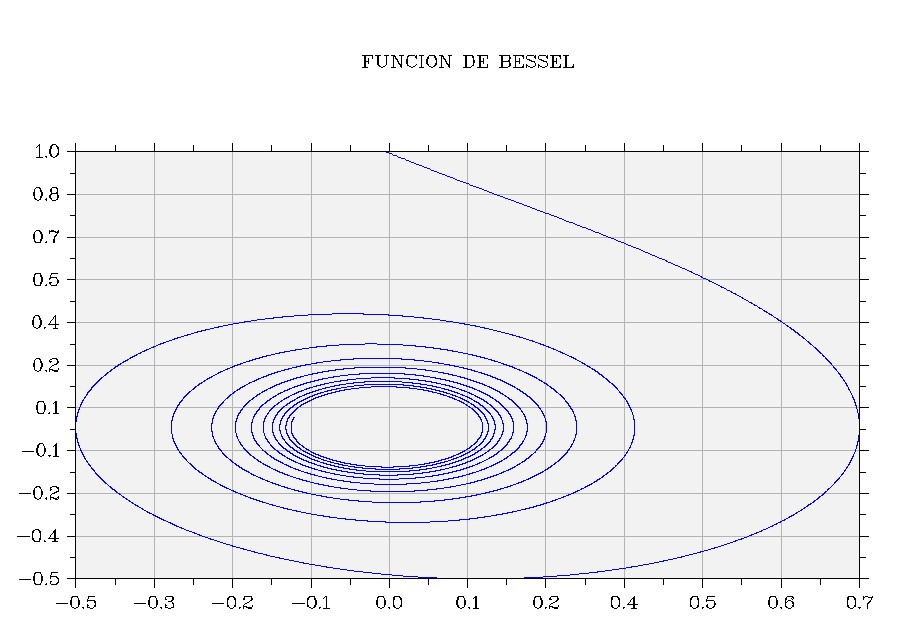
\includegraphics[width=1\textwidth]{Bessel.jpg}
	\caption{órbita de una ecuación de Bessel}
	\label{Bessel}
\end{figure}

\begin{figure}[H]
	\centering
	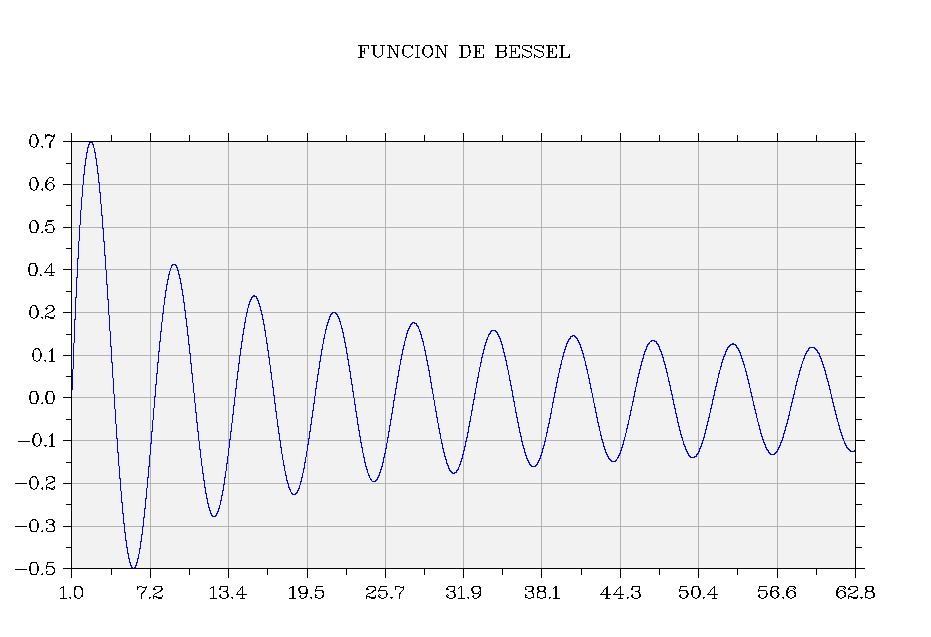
\includegraphics[width=1\textwidth]{Bessel_O.jpg}
	\caption{Función de Bessel en función del tiempo}
	\label{Bessel_O}
\end{figure}

	\newpage

\section{Propagador Armónico}
Otro de los modelos estudiados como paso previo a la resolución del problema planteado es el de un propagador armónico.

Este es un modelo sencillo, con una física más fácil de programar que la del proyecto propuesto, que servirá como prueba para las distintas metodologías y las herramientas presentadas en el apartado anterior. 

\subsection{Resultado de la Simulación}
%\begin{figure}[H]
%	\centering
%	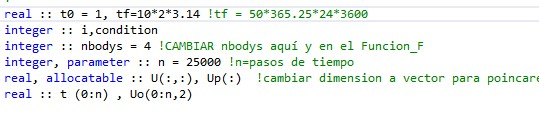
\includegraphics[width=1\textwidth]{armonio_CI.jpg}
%	\caption{Condiciones iniciales bajo las que se ha simulado el movimiento armónico}
	%\label{Armonico_CI}
%\end{figure}

\begin{figure}[H]
	\centering
	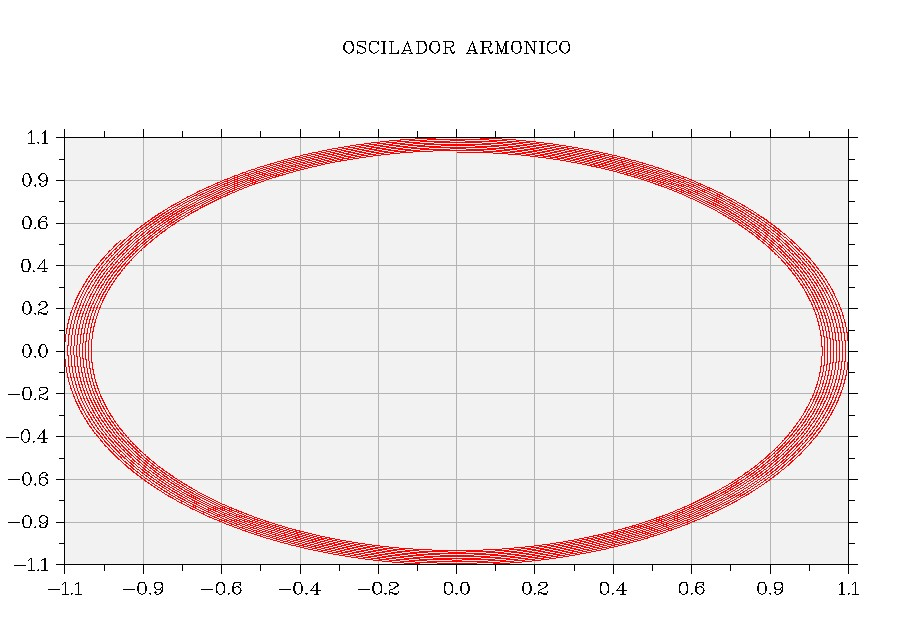
\includegraphics[width=1\textwidth]{armonio_EU.JPG}
	\caption{Órbita del oscilador armónico. Resultado de la simulación usando un propagador tipo Euler explicito}
	\label{Armonico_EU}
\end{figure}

\begin{figure}[H]
	\centering
	\includegraphics[width=1\textwidth]{Armonio_RG4.JPG}
	\caption{Órbita del oscilador armónico. Resultado de la Simulación utilizando un esquema numérico tipo Rungue-Kutta 4}
	\label{Armonico_RG4}
\end{figure}

\subsection{Conclusiones obtenidas de la simulación}

Tratándose de un sistema muy sencillo donde la solución es un coseno. Se puede observar que después de 10 periodos el esquema numérico de tipo Euler, provoca una divergencia de las órbitas creando una forma espiral, por otra parte el esquema numérico tipo Runge-Kutta ha conseguido mantener el resultado esperado. Todo esto es debido a que el esquema numérico Euler no es convergente ni estable dentro del domino del problema. De este primer y sencillo problema se determina que la elección del esquema numérico es determinante a la hora de poder simular satisfactoriamente un problema, pues nuestros resultados dependen del mismo, por ejemplo el estudio de la estabilidad de la solución de un problema de este carácter no podría ser llevado a cabo con un esquema numérico Euler, ya que de por sí el esquema sería inestable, incapacitando el estudio de estabilidad.

	\newpage

\section{N cuerpos}
Una vez realizado un análisis de un problema sencillo, como es el del propagador armónico, se pretende expandir todas las ideas implantadas en un modelo físico más complejo, como es el modelo de los N cuerpos.

El objetivo de realizar el estudio de este problema es comprobar que toda la metodología implementado en el propagador es aplicable a cualquier modelo físico, independientemente de la complejidad del mismo. Una vez se haya conseguido adaptar todo lo aprendido con el modelo sencillo al modelo de los N cuerpos la extrapolación de las herramientas a cualquier modelo físico, como el del cambio de órbita del satélite, será mucho más sencilla.

Para este problema se han realizado dos simulaciones distintas. En la primera se estudia el sistema Tierra-Luna-Satélite, que se asemeja al problema de los tres cuerpos donde la masa de un cuerpo es despreciable frente al resto. Dada la relevancia histórica de este problema se ha decidido estudiar el plano de Poincaré de este modelo y la estabilidad de Richardson. Por otra parte también se ha hecho una pequeña simulación de algunos de los planetas del sistema solar, para comprobar el funcionamiento del software para un mayor número de elementos.

\subsection{Sistema Tierra-Luna-Satélite}

Primero se empieza exponiendo los resultados obtenidos de distintas simulaciones donde se ha variado el tipo de esquema numérico y el tiempo total de simulación. Las condiciones iniciales del problema se recogen en la Figura \ref{TLS_CI}\\
\\ 

\begin{figure}[H]
	\centering
	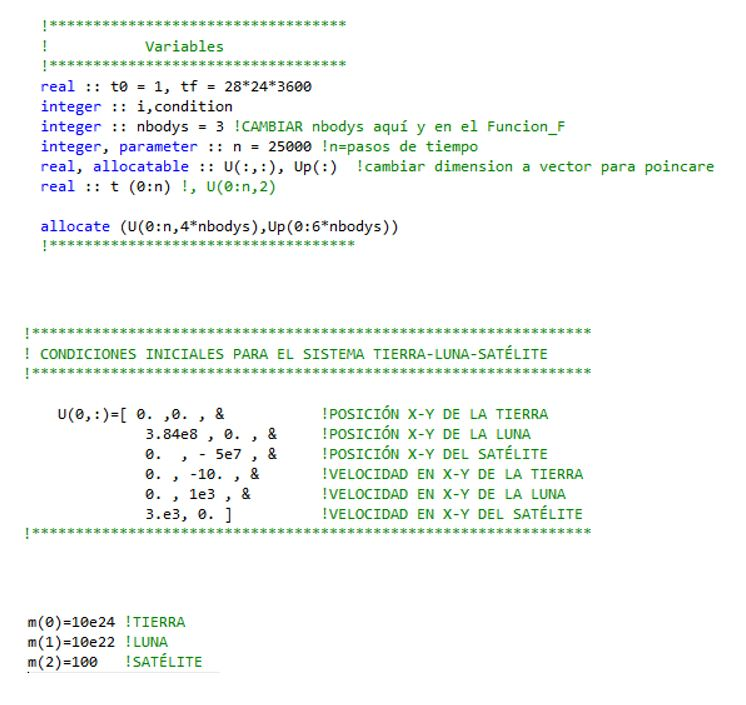
\includegraphics[width=0.8\textwidth]{TLS_CI.jpg}
	\caption{Condiciones iniciales bajo las que se ha simulado el sistema}
	\label{TLS_CI}
\end{figure}


\begin{figure}[H]
	\centering
	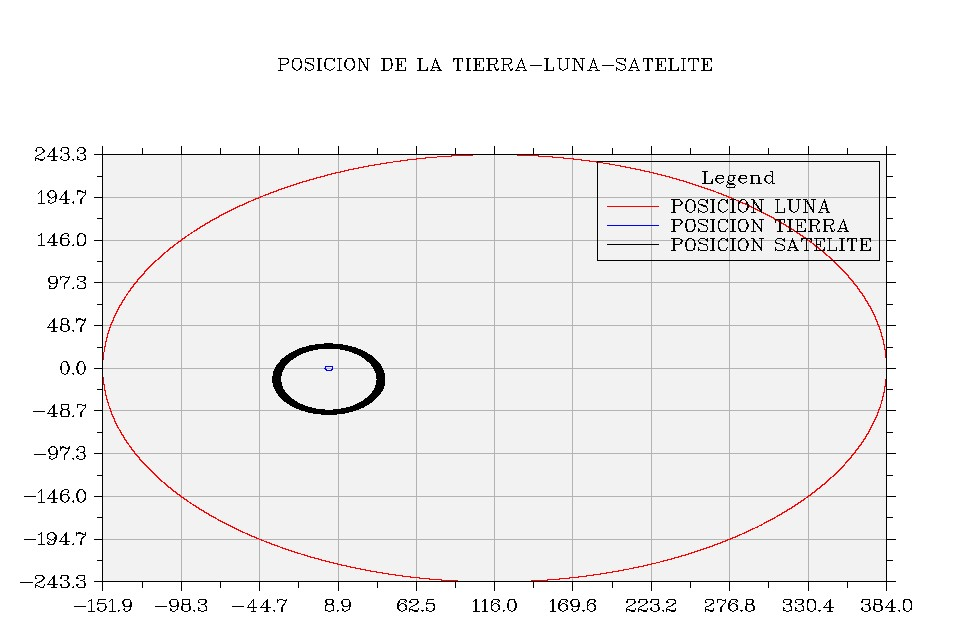
\includegraphics[width=1\textwidth]{TLS28D.jpg}
	\caption{Resultado de la Simulación utilizando un esquema numérico tipo Rungue-Kutta 4 para 28 días de simulación. Los valores se han dividido por $10^{6}$}
	\label{TLS28D_RG4}
\end{figure}

\begin{figure}[H]
	\centering
	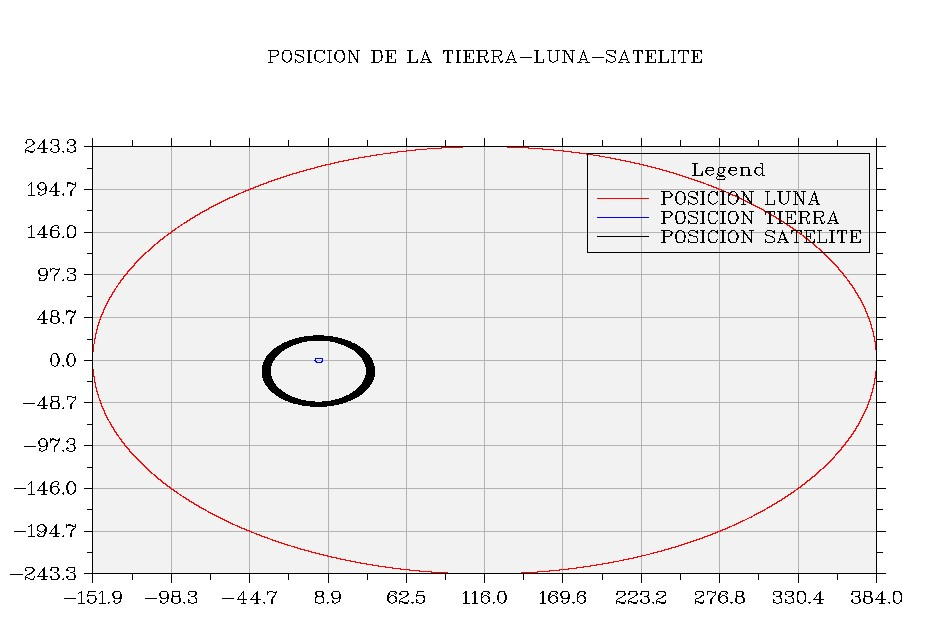
\includegraphics[width=1\textwidth]{TLS28D_RG2.jpg}
	\caption{Resultado de la Simulación utilizando un esquema numérico tipo Rungue-Kutta 2 para 28 días de simulación.  Los valores se han dividido por $10^{6}$}
	\label{TLS28D_RG2}
\end{figure}

\begin{figure}[H]
	\centering
	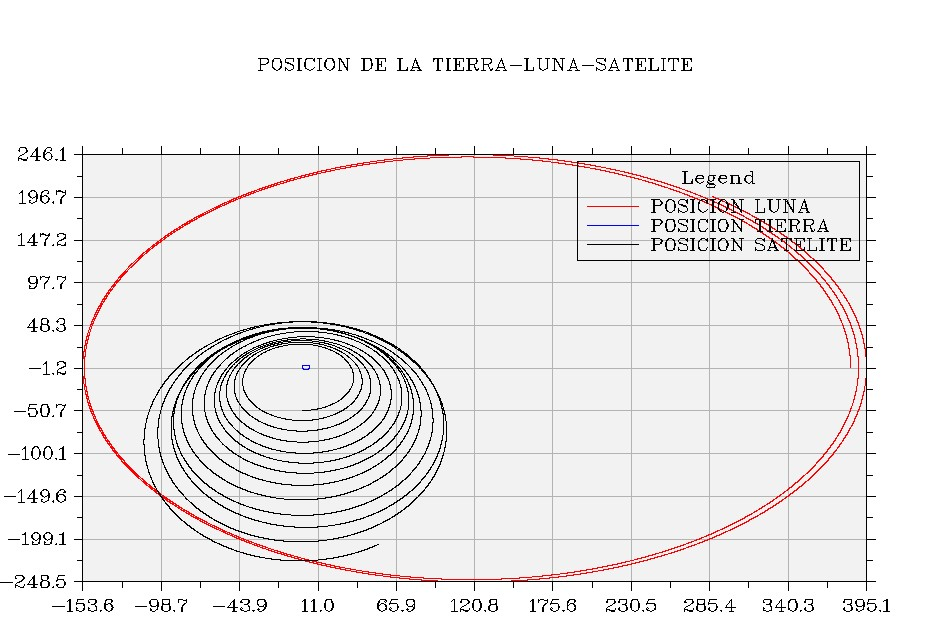
\includegraphics[width=1\textwidth]{TLS28D_EU.jpg}
	\caption{Resultado de la Simulación utilizando un esquema numérico tipo Euler para 28 días de simulación.  Los valores se han dividido por $10^{6}$}
	\label{TLS28D_EU}
\end{figure}


\begin{figure}[H]
	\centering
	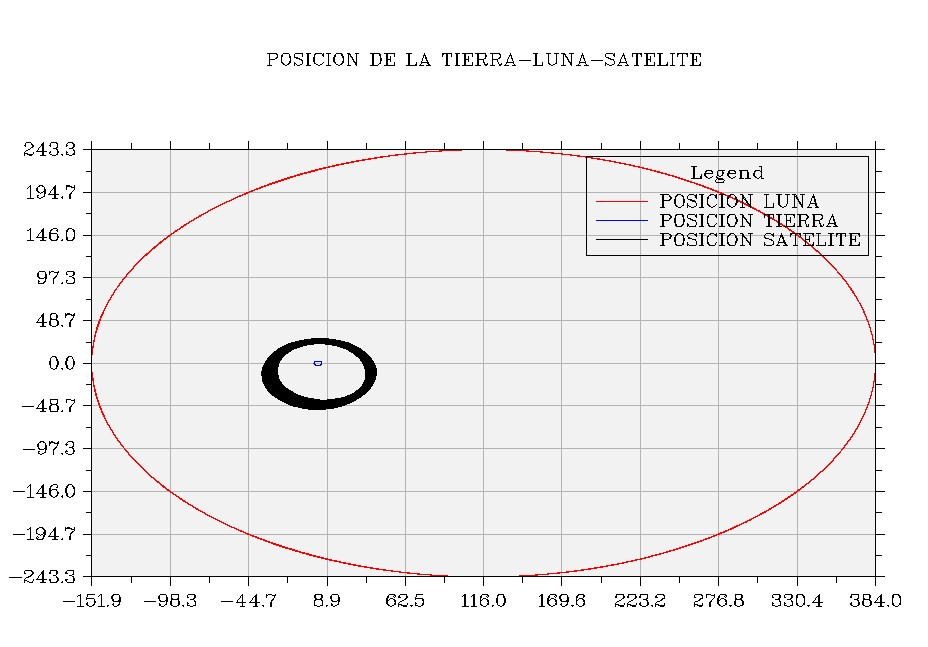
\includegraphics[width=1\textwidth]{TLS1A_RG4.jpg}
	\caption{Resultado de la Simulación utilizando un esquema numérico tipo Rungue-Kutta 4 para un año de simulación.  Los valores se han dividido por $10^{6}$}
	\label{TLS1A_RG4}
\end{figure}

\begin{figure}[H]
	\centering
	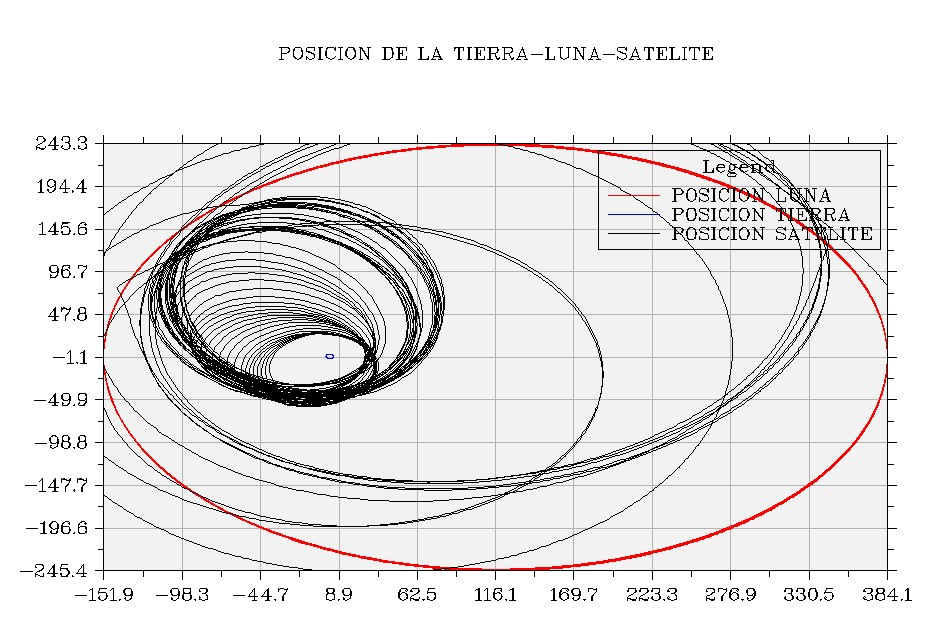
\includegraphics[width=1\textwidth]{TLS1A_RG2.jpg}
	\caption{Resultado de la Simulación utilizando un esquema numérico tipo Rungue-Kutta 2 para un año de simulación.  Los valores se han dividido por $10^{6}$}
	\label{TLS1A_RG2}
\end{figure}

\begin{figure}[H]
	\centering
	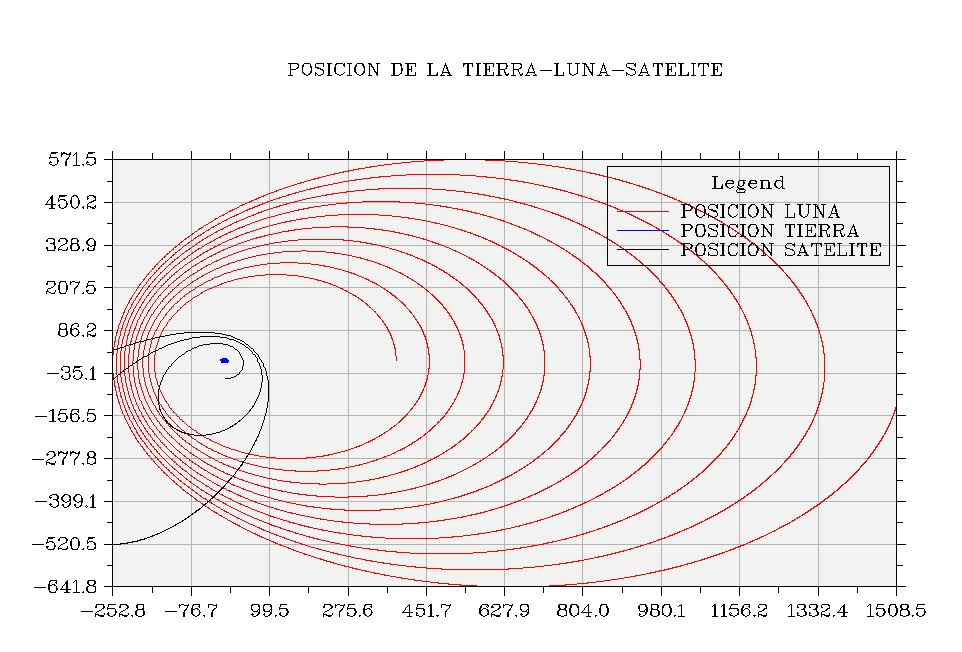
\includegraphics[width=1\textwidth]{TLS1A_EU.jpg}
	\caption{Resultado de la Simulación utilizando un esquema numérico tipo Euler para un año de simulación.  Los valores se han dividido por $10^{6}$}
	\label{TLS1A_EU}
\end{figure}

Como se puede observar, y se ha comentado anteriormente, la elección del tipo de esquema numérico es fundamental. Observando las figuras se aprecia que el mejor esquema numérico para simular estos sistemas es el Runge-Kutta de orden 4, Por lo tanto en los siguientes puntos se usará el esquema numérico Runge-Kutta 4. Un punto a destacar es que el satélite no describe una órbita perfectamente circular como podría esperarse \textit{a priori} por lo tanto este objeto va ser el próximo elemento de estudio. Para analizar más en detalle este aspecto se ha realizado el plano de Poincaré. En este punto se han simulado varias órbitas para distintas condiciones iniciales obteniéndose un mapa de puntos distinto para cada condición inicial. También se ha representado el plano de Poincaré variando la cantidad de tiempo simulado.

\begin{figure}[H]
	\centering
	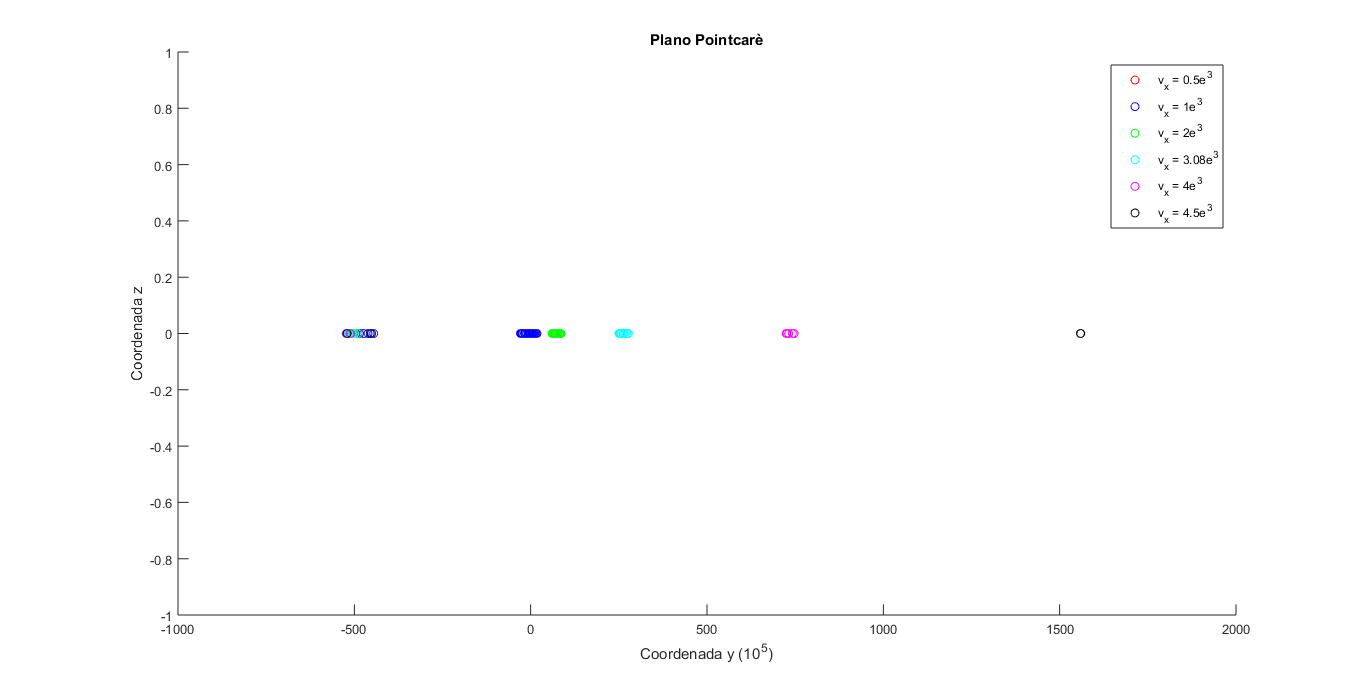
\includegraphics[width=1\textwidth]{PointCareCI_1.png}
	\caption{Intersección de la órbita en el plano de Poincaré variando las condiciones iniciales:1}
	\label{PointCareCI_1}
\end{figure}

\begin{figure}[H]
	\centering
	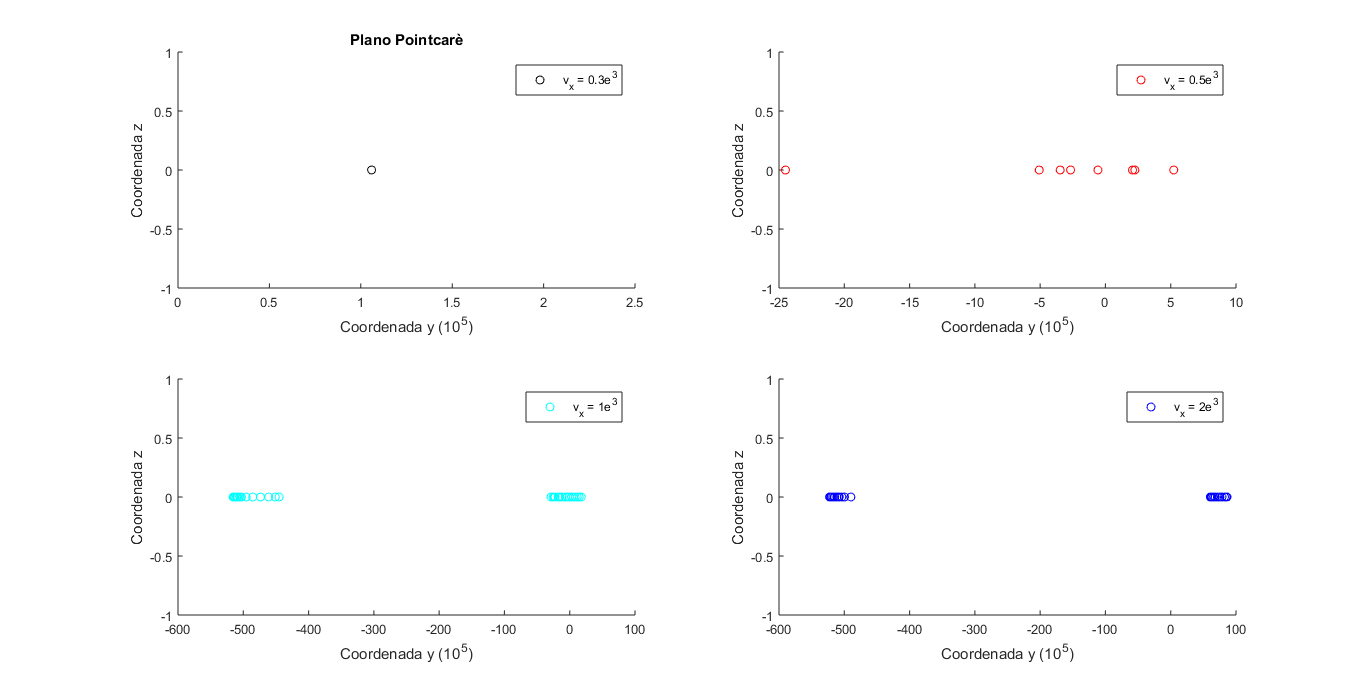
\includegraphics[width=1\textwidth]{PointCareCI_2.png}
	\caption{Intersección de la órbita en el plano de Poincaré variando las condiciones iniciales:2}
	\label{PointCareCI_2}
\end{figure}

\begin{figure}[H]
	\centering
	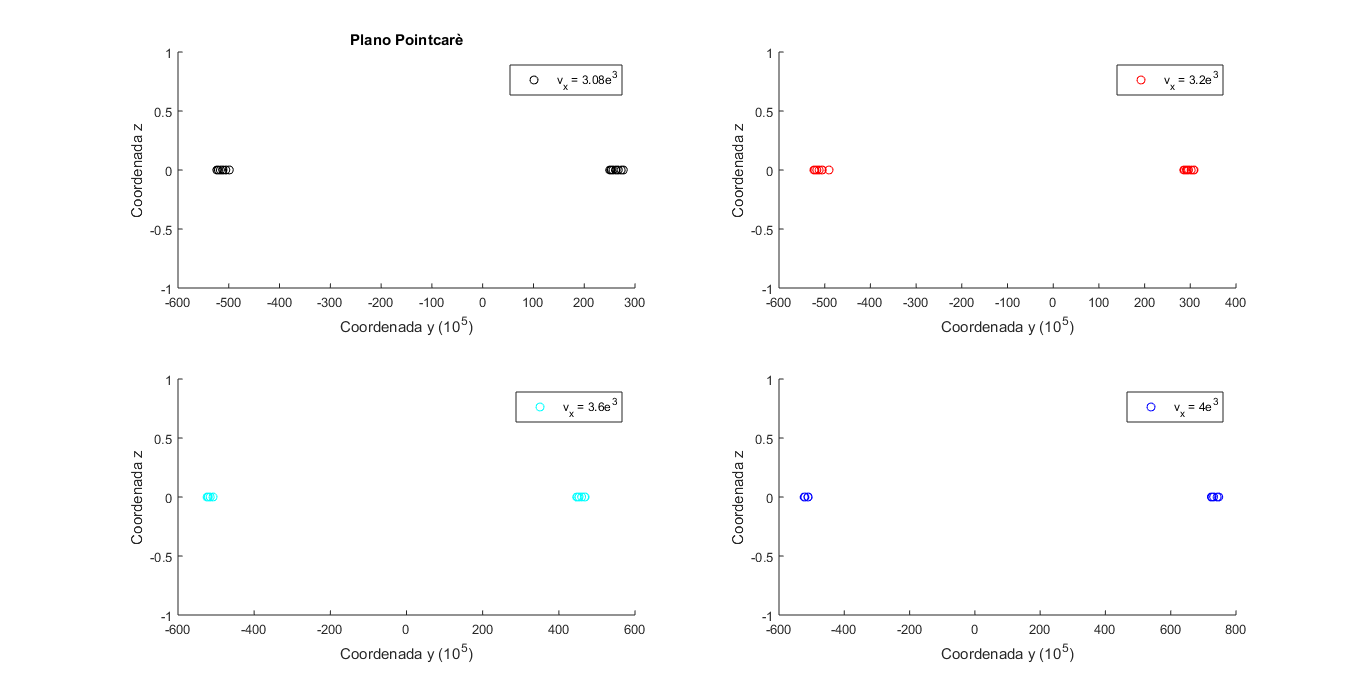
\includegraphics[width=1\textwidth]{PointCareCI_3.png}
	\caption{Intersección de la órbita en el plano de Poincaré variando las condiciones iniciales:3}
	\label{PointCareCI_3}
\end{figure}

\begin{figure}[H]
	\centering
	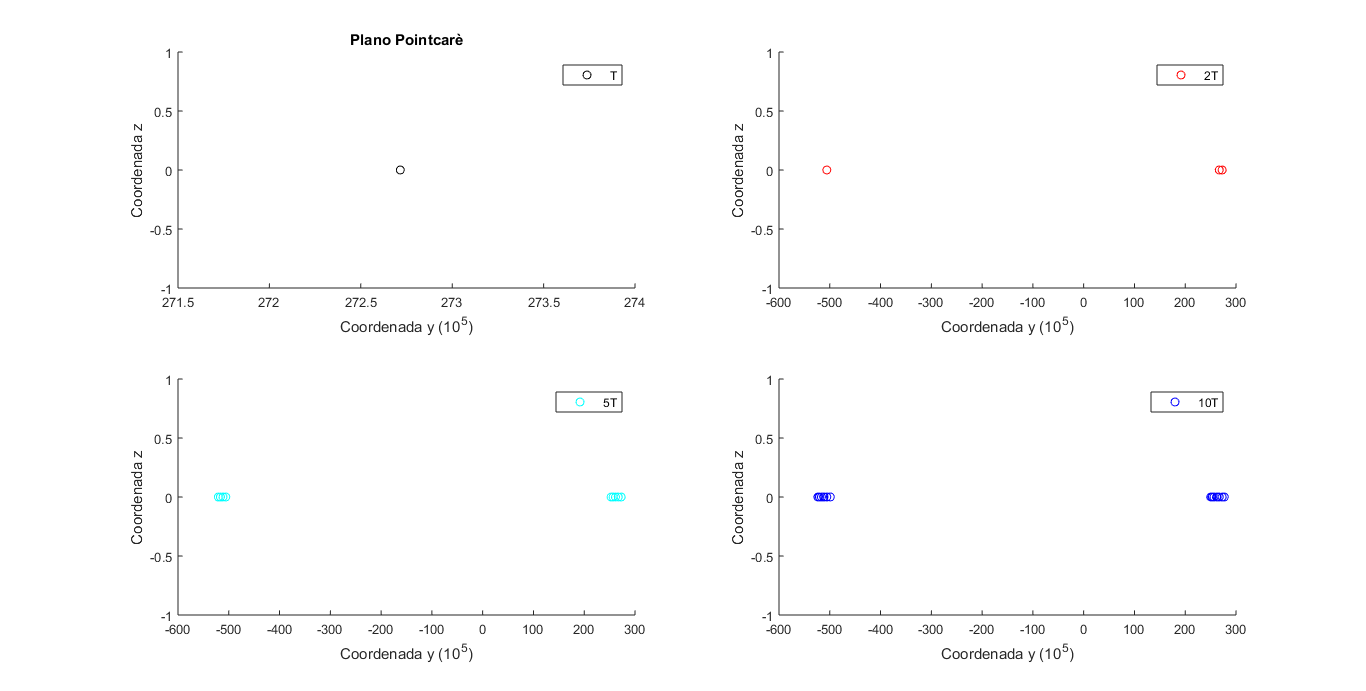
\includegraphics[width=1\textwidth]{PointCareT_1.png}
	\caption{Intersección de la órbita en el plano de Poincaré aumentado la cantidad de periodos simulados}
	\label{PointCareT_1}
\end{figure}

\begin{figure}[H]
	\centering
	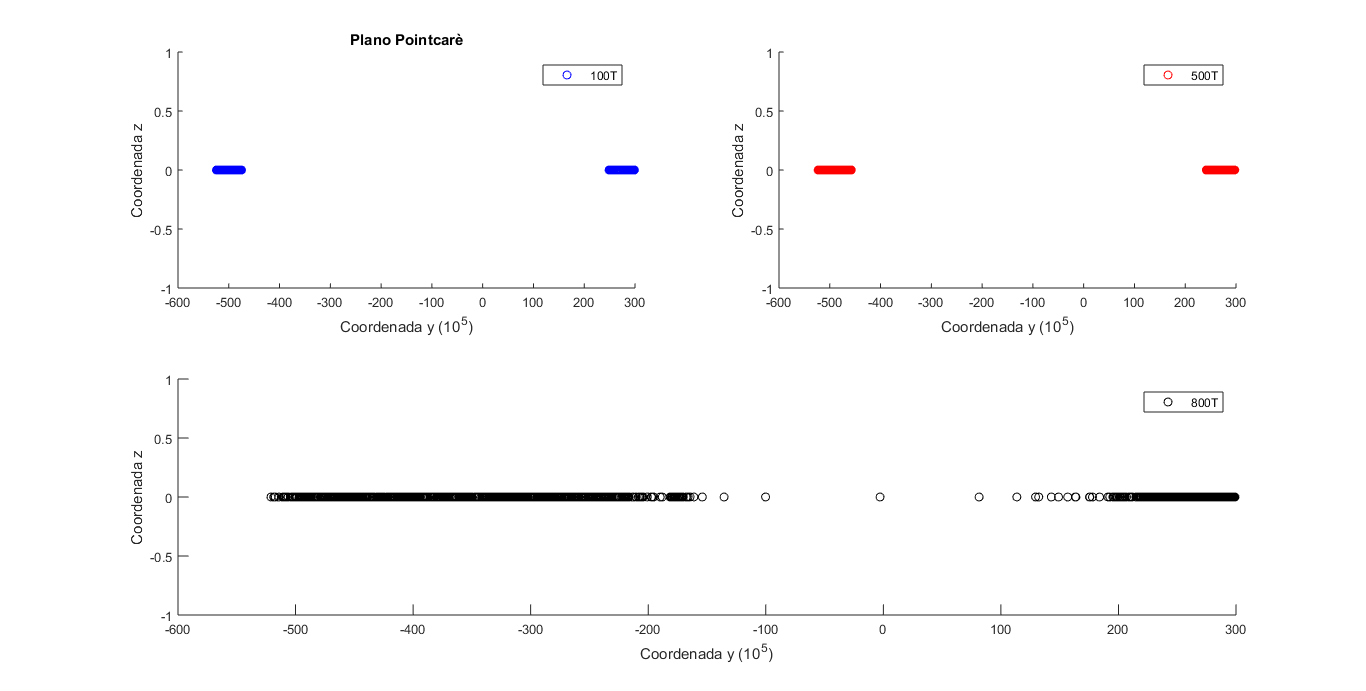
\includegraphics[width=1\textwidth]{PointCareT_2.png}
	\caption{Intersección de la órbita en el plano de Poincaré aumentado la cantidad de periodos simulados}
	\label{PointCareT_2}
\end{figure}


A la vista de las gráficas se aprecia que el plano de Poincaré varía tanto con las condiciones iniciales como con los periodos simulados. A su vez, se aprecia que en un mismo plano hay dos regiones de puntos, una en la zona negativa y otra en la positiva. Esto se debe a la forma elíptica de las soluciones, lo que provoca que haya dos puntos de intersección con el plano con cada vuelta, un punto en la zona del semieje negativo y el otro en la zona del semieje positivo.

\newpage
\subsection{Sistema Solar}
 
Esta simulación se ha llevado acabo simulando ciertos elementos dentro del sistema solar entre ellos se encuentra: el Sol, la Tierra, la Luna y Marte. Las condiciones iniciales de dicha simulación se recogen en la Figura \ref{TLMS_CI}

\begin{figure}[H]
	\centering
	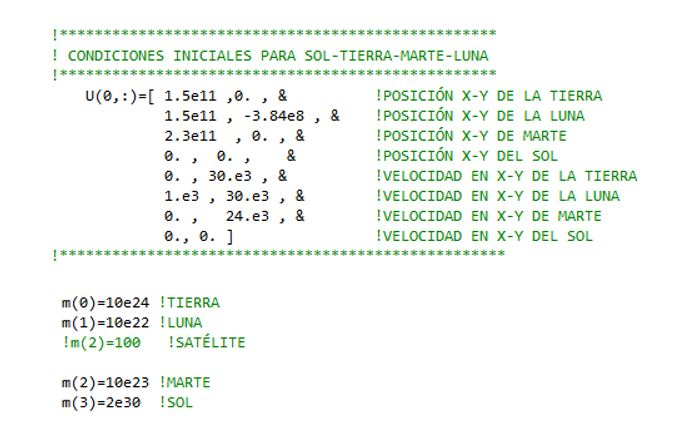
\includegraphics[width=0.8\textwidth]{TLMS_CI.jpg}
	\caption{Condiciones iniciales bajo las que se ha simulado el sistema}
	\label{TLMS_CI}
\end{figure}


\begin{figure}[H]
	\centering
	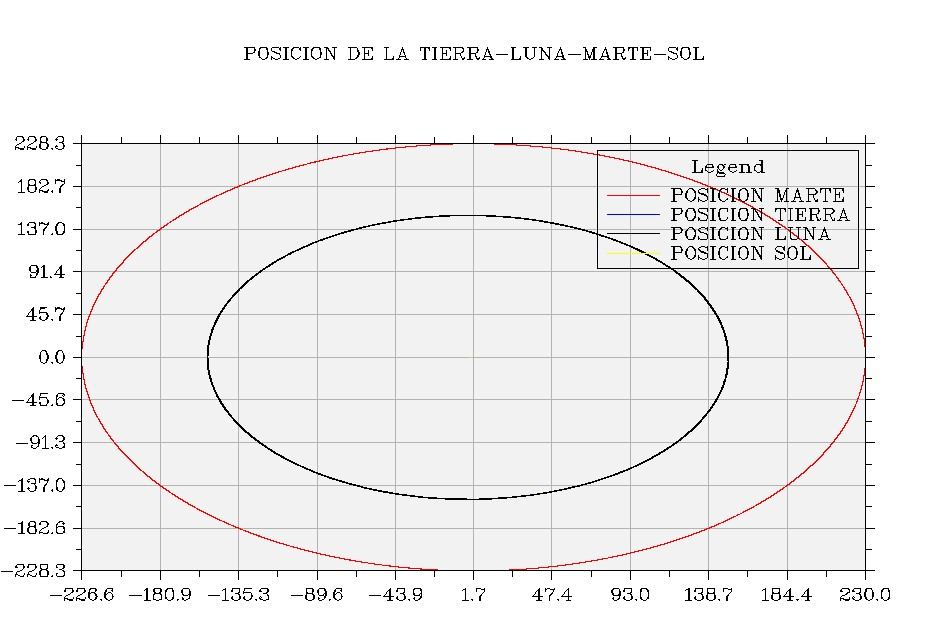
\includegraphics[width=1\textwidth]{TLMS10A_RG4.jpg}
	\caption{Resultado de la Simulación utilizando un esquema numérico tipo Runge-Kutta 4 para 10 años de simulación.  Los valores se han dividido por $10^{6}$}
	\label{TLMS10A_RG4}
\end{figure}

\begin{figure}[H]
	\centering
	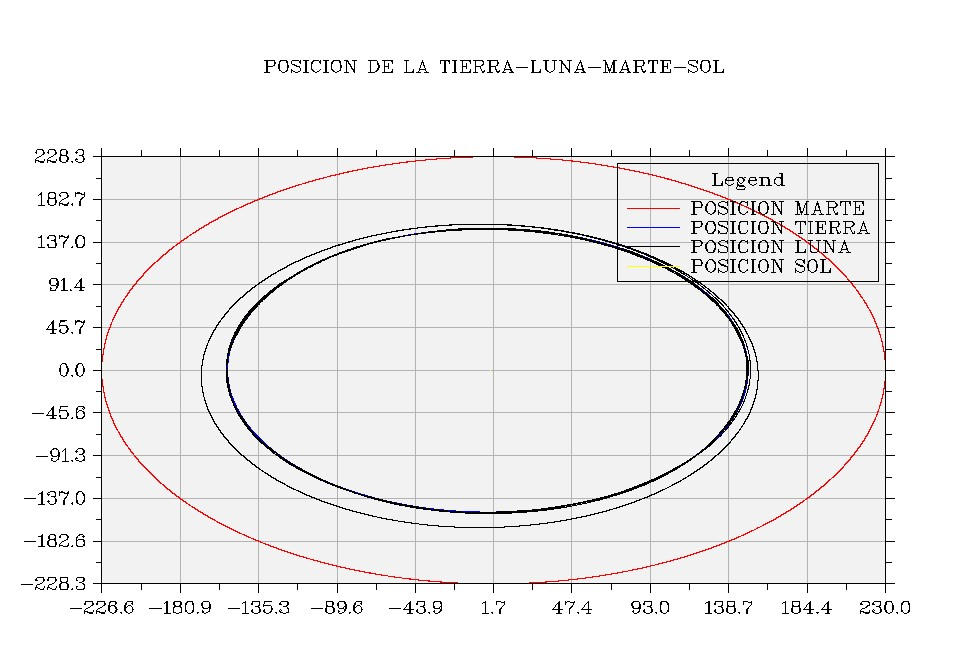
\includegraphics[width=1\textwidth]{TLMS10A_RG2.jpg}
	\caption{Resultado de la Simulación utilizando un esquema numérico tipo Rungue-Kutta 2 para 10 años de simulación.  Los valores se han dividido por $10^{6}$}
	\label{TLMS10A_RG2}
\end{figure}

\begin{figure}[H]
	\centering
	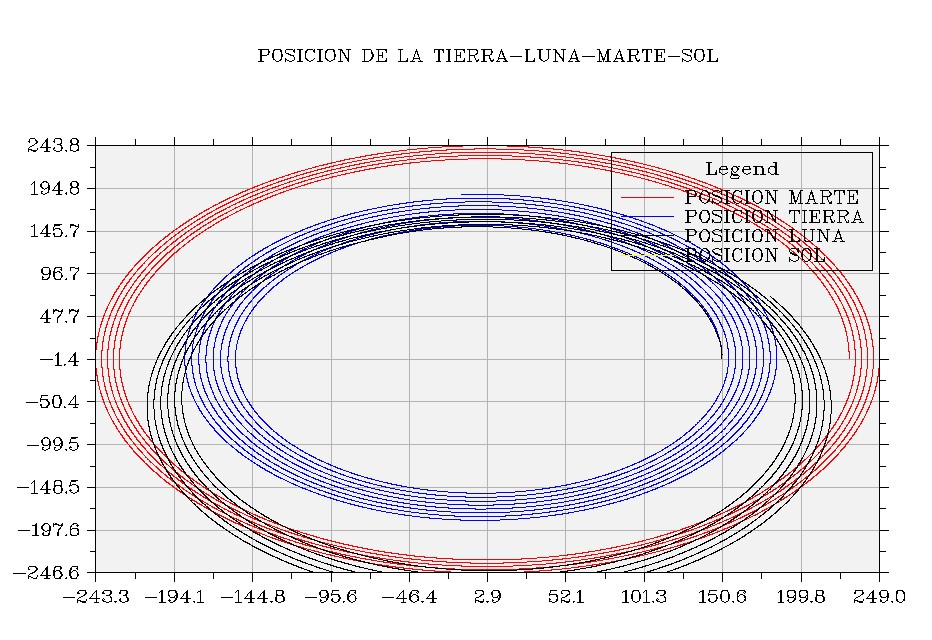
\includegraphics[width=1\textwidth]{TLMS10A_EU.jpg}
	\caption{Resultado de la Simulación utilizando un esquema numérico tipo Euler para 10 años de simulación.  Los valores se han dividido por $10^{6}$}
	\label{TLMS10A_EU}
\end{figure}


\begin{figure}[H]
	\centering
	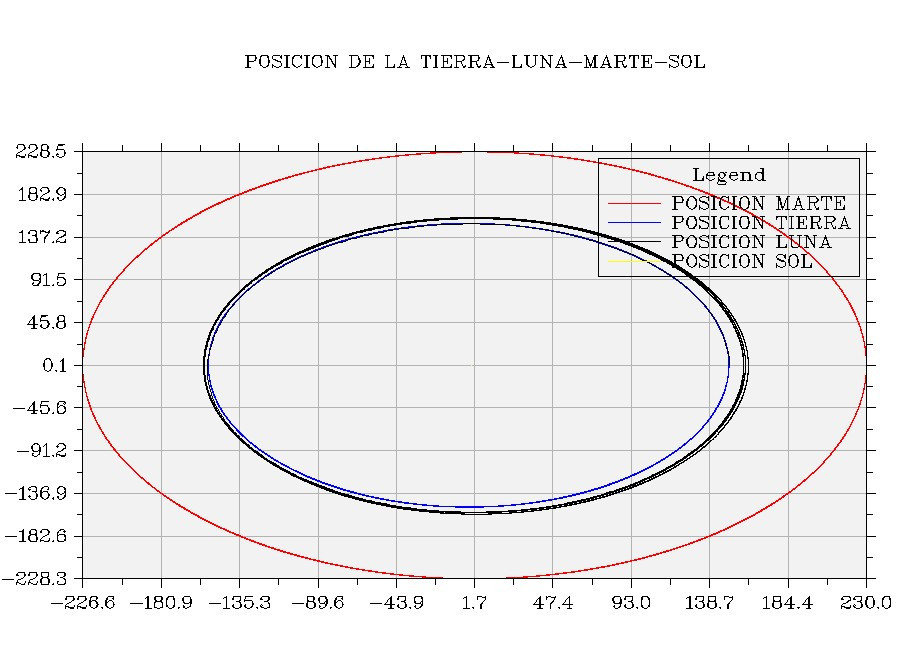
\includegraphics[width=1\textwidth]{TLMS50A_RG4.jpg}
	\caption{Resultado de la Simulación utilizando un esquema numérico tipo Rungue-Kutta 4 para 50 años de simulación.  Los valores se han dividido por $10^{6}$}
	\label{TLMS50A_RG4}
\end{figure}

\begin{figure}[H]
	\centering
	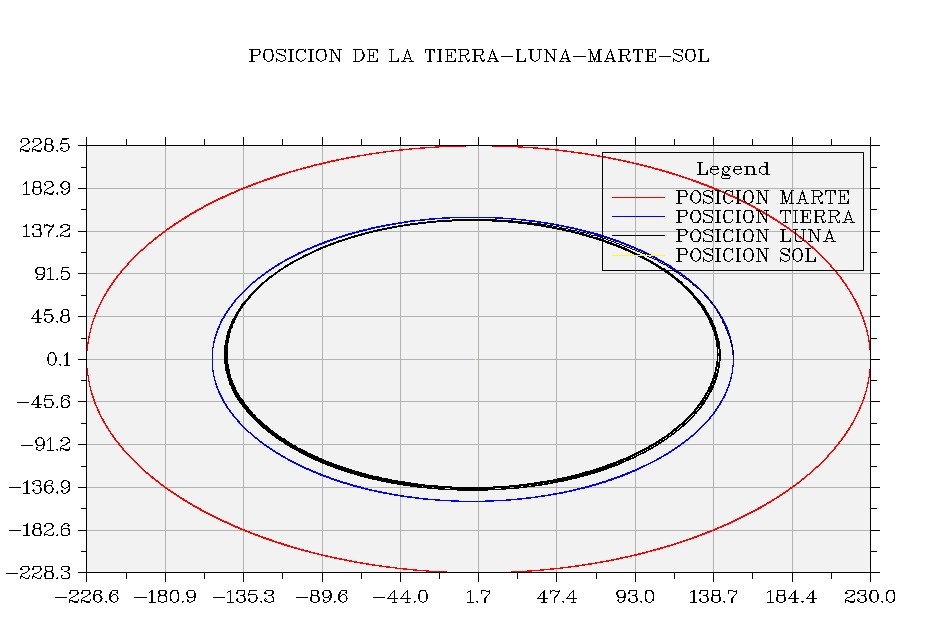
\includegraphics[width=1\textwidth]{TLMS50A_RG2.jpg}
	\caption{Resultado de la Simulación utilizando un esquema numérico tipo Rungue-Kutta 2 para 50 años de simulación.  Los valores se han dividido por $10^{6}$}
	\label{TLMS50A_RG2}
\end{figure}

\begin{figure}[H]
	\centering
	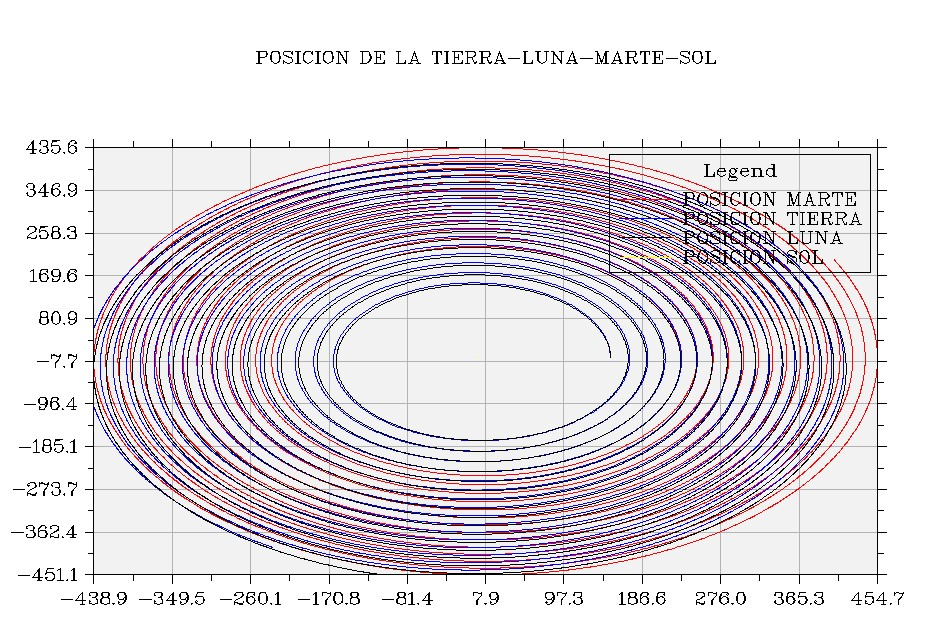
\includegraphics[width=1\textwidth]{TLMS50A_EU.jpg}
	\caption{Resultado de la Simulación utilizando un esquema numérico tipo Euler para 50 años de simulación.  Los valores se han dividido por $10^{6}$}
	\label{TLMS50A_EU}
\end{figure}

De nuevo, la solución obtenida con el esquema de tipo Euler diverge con mayor facilidad que la de Runge-Kutta. Además, en este caso, para una simulación de 50 años se empieza a apreciar una variación significativa en el esquema más preciso, el Runge-Kutta 4. Esto nos hace ver que para simular correctamente este sistema sería necesario implementar un esquema numérico de mayor orden, que permita corregir dicha desviación para tiempos grandes.
	\newpage
	
\section{Cambio de órbita de un satélite}
Para finalizar el análisis realizado a lo largo de este informe se retoma el problema principal del cambio de órbita de un satélite. En concreto, el objetivo principal es estimar el impacto del fallo del sistema de apagado del motor electrostático sobre la órbita final obtenida.

En el caso de que el sistema de apagado del motor no funcione correctamente y el motor no se detenga cuando corresponde, la órbita obtenida por el satélite será diferente a la que se quería obtener en un inicio. En esta parte del informe se estudiará la variación de la órbita final en el caso de que el motor no se apague.

\subsection{Simulación}
Se ha decidido utilizar un caso muy sencillo donde se observa la evolución de la órbita a lo largo del tiempo. variando entre las distintas simulaciones el valor de empuje máximo que proporciona el sistema de propulsión. Para estas simulaciones se considera que satélite se encuentra en una órbita inicial que es circular, alrededor de la tierra, con una masa seca de 1000 kg y 200 kg de combustible. El impulso especifico es de 2000 s. El esquema numérico usado para la simulación es el Runge-Kutta 4 y se simula para un tiempo igual a 100 periodos de la órbita nominal.

\begin{figure}[H]
	\centering
	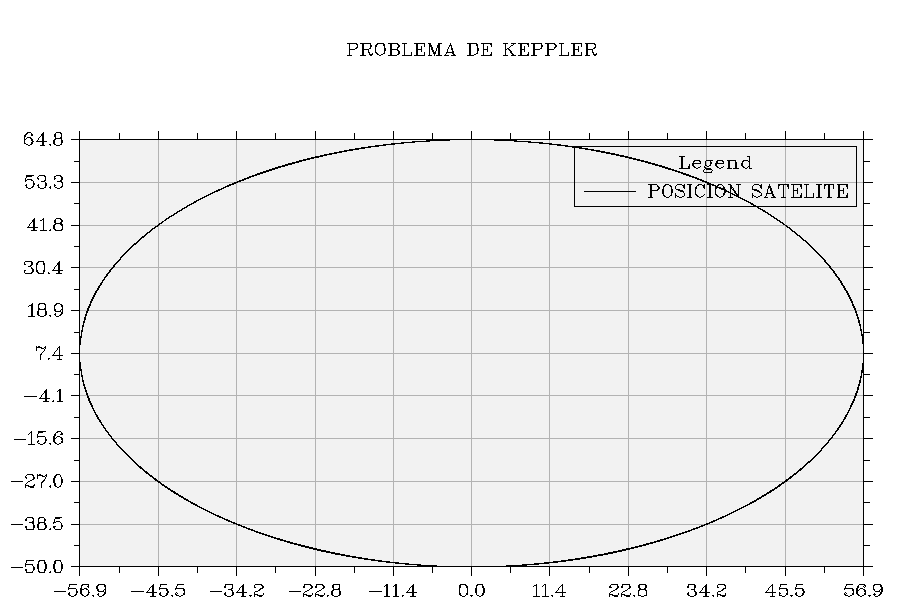
\includegraphics[width=1\textwidth]{E=0_100T.png}
	\caption{Resultado de la Simulación con motor parado (condiciones iniciales)}
	\label{E=0}
\end{figure}

\begin{figure}[H]
	\centering
	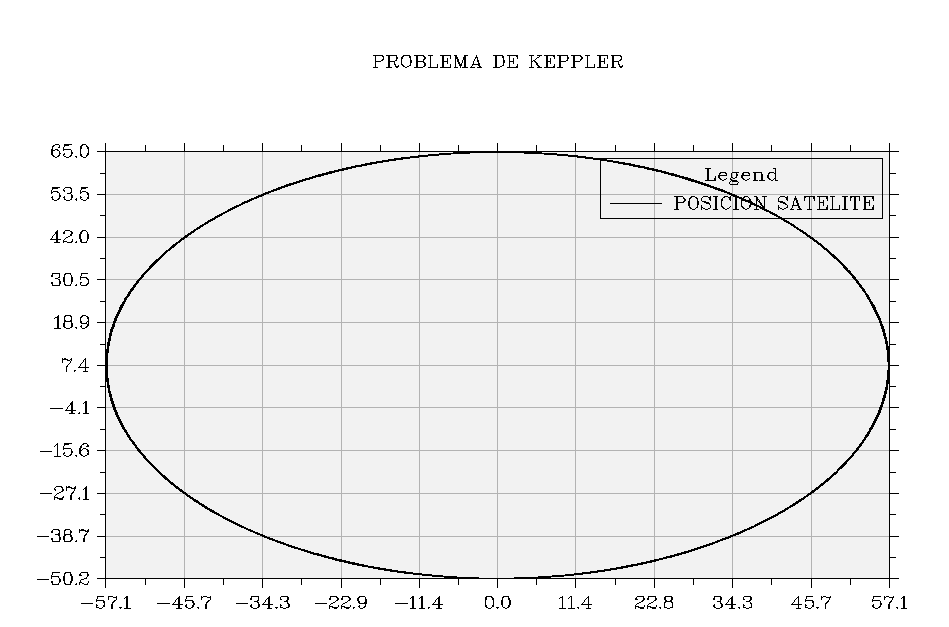
\includegraphics[width=1\textwidth]{E0001_100T.PNG}
	\caption{Resultado de la Simulación con un empuje máximo de 0.001 N}
	\label{E=0.001}
\end{figure}

\begin{figure}[H]
	\centering
	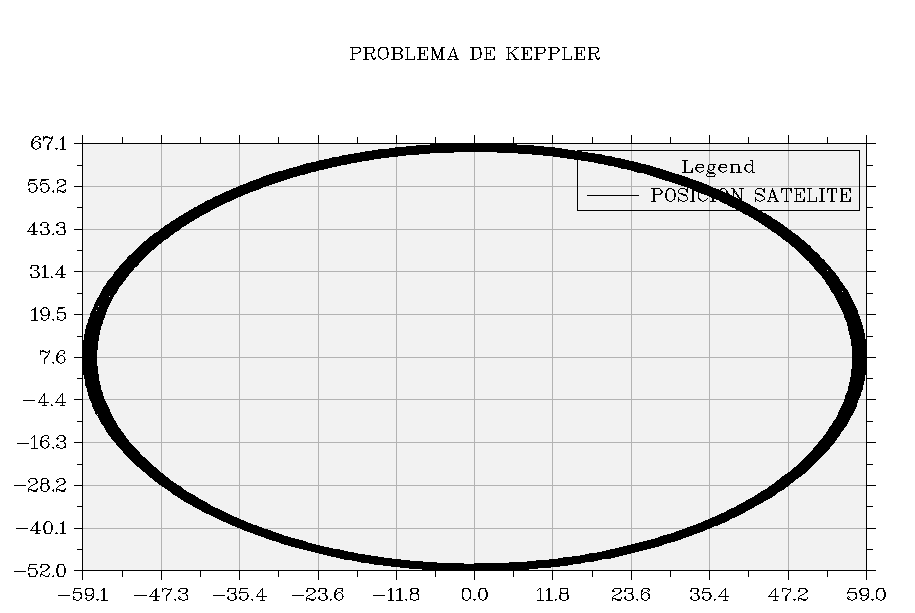
\includegraphics[width=1\textwidth]{E001_100T.PNG}
	\caption{Resultado de la Simulación con un empuje máximo de 0.01 N}
	\label{E=0.01}
\end{figure}

\begin{figure}[H]
	\centering
	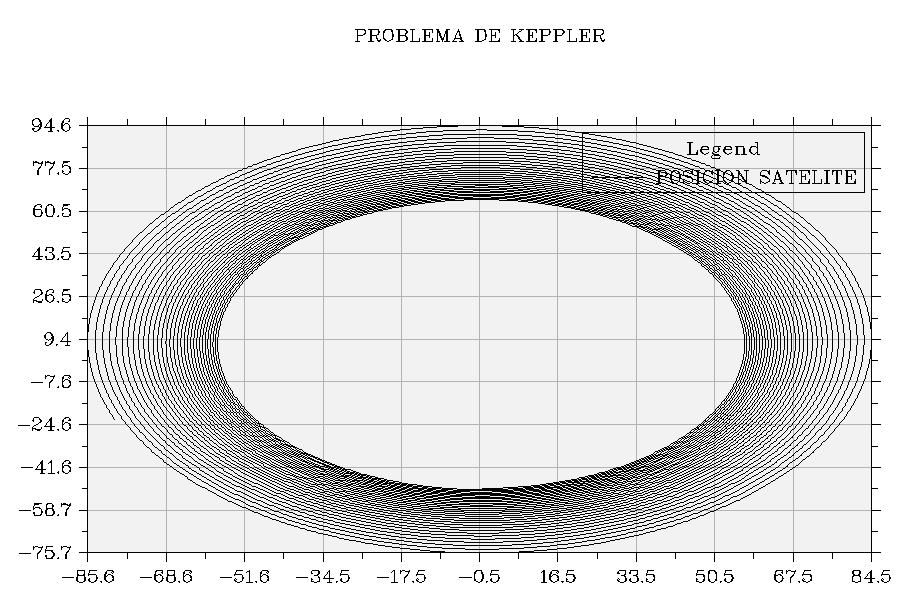
\includegraphics[width=1\textwidth]{E01_100T.PNG}
	\caption{Resultado de la Simulación con un empuje máximo de 0.1 N}
	\label{E=0.1}
\end{figure}

\begin{figure}[H]
	\centering
	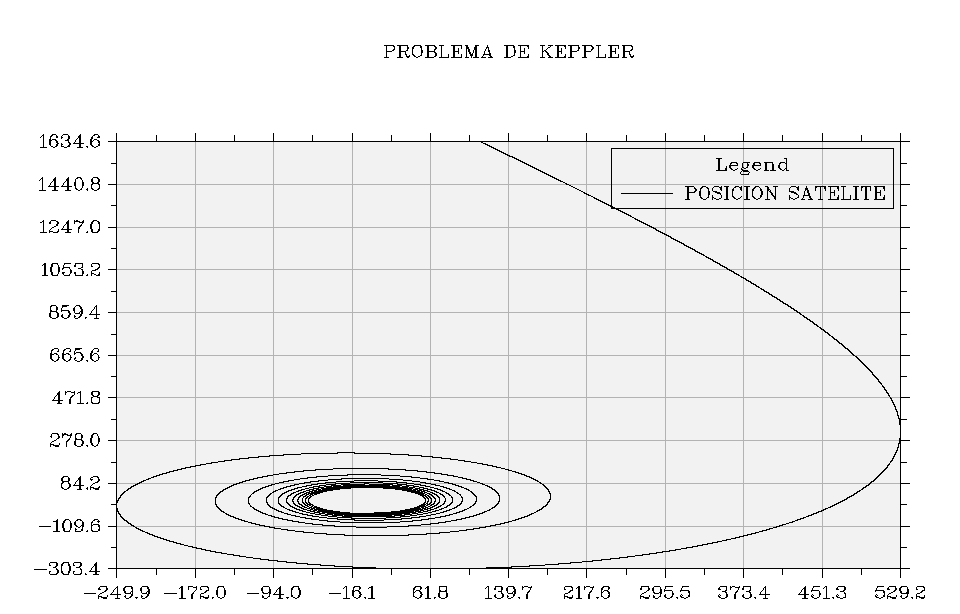
\includegraphics[width=1\textwidth]{E05_100T.PNG}
	\caption{Resultado de la Simulación con un empuje máximo de 0.5 N}
	\label{E=0.5}
\end{figure}

\begin{figure}[H]
	\centering
	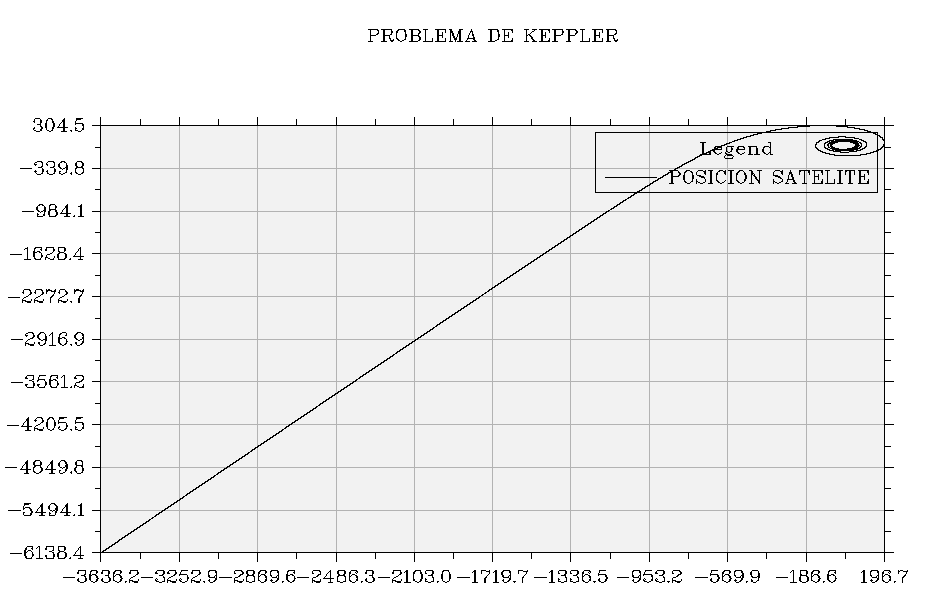
\includegraphics[width=1\textwidth]{E1_100T.PNG}
	\caption{Resultado de la Simulación con un empuje máximo de 1 N}
	\label{E=1}
\end{figure}

\subsection{Conclusión}
Como se pude observar la órbita del vehículo va creciendo debido al empuje que proporciona el motor, en los primeros casos dado que el empuje del motor es muy pequeño el satélite se mantiene en órbita alrededor de la tierra pero según se aumenta el empuje máximo esta órbita cada vez llega más lejos de la tierra hasta que adquiere la velocidad de escape y se aleja hacia el infinito a través de una hipérbola.
En el análisis del problema estudiado, el del fallo en el sistema de apagado del motor, esto implica que si el motor tiene un empuje bajo, como es el caso de un motor electrostático, el no apagado del motor provocará la variación, significativa, de la órbita, pero manteniéndose dentro de la zona de influencia de la Tierra y permitiendo nuevas maniobras de corrección para alcanzar la órbita deseada. 
En el caso de disponer de un motor con un empuje nominal mayor, a partir de 0.5N, el no apagado del motor podría llegar a provocar la salida de la zona de influencia y la pérdida efectiva, sin posibilidad de reinserción, del satélite. 

	\newpage
	
\section{Conclusiones}
\begin{itemize}
	\item Se ha conseguido desarrollar de manera satisfactoria en FORTRAN un programa que es capaz de \textbf{resolver cualquier problema de EDOS de condiciones iniciales}, siempre y cuando se introduzca la función problema dentro del archivo pertinente. También se tienen que tener en cuenta la limitaciones existentes debido a los pocos esquemas numéricos que hay implementados.
	\item La selección del tipo de esquema numérico es  importante, ya que una mala elección del tipo de esquema numérico puede desembocar en una solución errónea. Antes de empezar a simular cualquier problema conviene estudiar el tipo de sistema para seleccionar un esquema numérico acorde a lo que se quiere realizar. En el caso de los problemas propuesto a lo largo de este informe los esquemas numéricos del tipo Runge-Kutta han demostrado generar soluciones más precisas que los de tipo Euler. Por tanto, para problemas de órbitas es necesario utilizar \textbf{esquemas numéricos de alto orden} para conseguir \textbf{convergencia numérica} para tiempos de integración largos. El mayor orden que se ha utilizado en el trabajo es un Runge-Kutta de orden 4, que en ocasiones ha resultado insuficiente, sobretodo cuando se propagan muchos periodos. 
	\item La distribución en funciones de los distintos elementos utilizados en los programas permite variar las funciones analizadas, los integradores y la evolución temporal de manera sencilla.
\end{itemize}

\section*{ANEXO I: SOFTWARE}
En este apartado se realizará una breve explicación de los distintos módulos que se utilizan en el programa.

\begin{itemize}
\item \textbf{MAIN EDOS}: Corresponde al programa principal, el cual, utilizará el resto de módulos. En este programa se definirá la partición temporal, se impondrán las condiciones iniciales del problema de \textit{EDOS}, y se hará la llamada a las subrutinas que resuelven el porblema de ecuaciones diferenciales ordinarias. Como se puede observar en la siguiente figura, la llamada al resolvedor del problema de Cauchy implica 4 argumentos: la pertición temporal, el operador direrencial correspondiente al problema que se quiere integrar (NBodies, OsciladorArmónico, FunciónBessel, etc...), el esquema numérico que se quiere emplear y la matriz que guarda las soluciones del problema para cada paso de tiempo (U).

\begin{figure}[H]
	\centering
	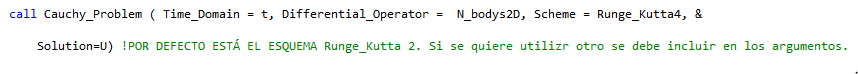
\includegraphics[width=1\textwidth]{call_CProblem.PNG}
	\caption{Llamada al resolvedor del problema de Cauchy}
	%\label{E=1}
\end{figure}

\item \textbf{FuncionF}: este módulo guarda en subrutinas todos los problemas que se desee integrar. En concreto se han programado 5 problemas: función de Bessel, Oscilador Armónico, problema de Keppler, problema de los N cuerpos en 2 dimensiones y el problema de los N cuerpos en 3 dimensiones. 

\item \textbf{StateVectorEvolution}: Contiene el módulo \textit{TemporalSchemes}. Se han programado los esquemas numéricos que se han empleado: Euler explícito, Runge-Kutta2 y Runge-Kutta4. Cabe destacar que los bucles que recorren todos los pasos temporales se han introducido en cada esquema numérico y no en el programa principal. Se ha programado un \textit{abstract interface} para poder utilizar en todos los esquemas la función F relativa a cada problema. 

\item \textbf{ODEInterface}: En este módulo se ha definido un \textit{abstract interface} para poder caracterizar las funciones F que definen cada problema. Esto se utiliza para definir completamente la forma que tienen las funciones F que se van a integrar y facilita la implementación y entendimiento del código. En el módulo StateVectorEvolution, se implementará un \textit{procedure} (una única vez) para que todos los esquemas numéricos utilicen la función F del sistema de forma que se encuentre totalmente caracterizada matemáticamente. De esta forma se asegurará que la función del sistema sea del mismo orden que el vector de estado asociado a cada problema.

\item \textbf{dislinmod}: Este módulo es un \textit{wraper} realizado por el compañero Imanol Sardón Delgado (quien nos ha permitido usar su código y nos ha ayudado a implementarlo), que se ha utilizado para facilitar el uso de la herramienta gráfica \textit{dislin}.


\end{itemize}


\end{document}
